% 1. 多智能体合作任务中常常关注部分可观测,非平稳性和信用分配等问题,而动态目标问题同样重要,例如,在经典的分手厨房游戏中,智能体完成的订单需要匹配用户的需求,同样的订单在分别在时间步1和时间步2送出,可能得到是奖励和惩罚。当前的合作MARL环境中尚未考虑动态目标的问题,流行的overcookedAI也是如此。
% 2. 动态任务目标问题很难,因为在MARL问题中加入了优化目标的随机性,优化目标改变时,智能体已经学到的策略却无法得到既定奖励,甚至得到惩罚,这会导致策略梯度朝着与目标改变之前相反的方向更新网络的权重,但是这个问题从直觉上而言是MARL可以解决的,因为在完全可观测的博弈环境中,目标变化时环境的state发生改变,这对智能体是已知的。
% 3. ComplexOvercooked和overcooked\_ai的对比, 列表,并简单介绍我们的环境
% 4. 我们的贡献可以总结如下:
% 1. 我们提出了一个多智能体强化学习的环境, ComplexOvercooked,这个环境还原了真实游戏的配置,对用户很友好并且易于配置,有利于拓展合作智能体的能力边界。
% 2.我们在ComplexOvercooked配置了键盘、智能体,和LLM的控制接口,可以轻易地收集人类玩家的数据,便于人机合作算法以及合作大模型算法的研究。
% 3. 我们在多个自定义的ComplexOvercooked布局中测试了经典MARL算法的性能,证实了在该环境中增强MARL算法性能的潜力。
In multi-agent cooperative tasks, significant attention is often given to issues such as partial observability\cite{zhu2022survey}, non-stationarity\cite{papoudakis2019dealing}, and credit assignment \cite{wang2021towards}. However, the challenge of dynamic objectives is equally important. For example, in the classic Overcooked game, the orders completed by agents must match user demands. The same order, if delivered at timestep $t_1$ versus timestep $t_2$, may result in either a reward or a penalty. Current cooperative MARL environments, including the popular \textit{Overcooked-AI} \cite{carroll2019utility}, have yet to address the challenge of dynamic objectives.

The problem of dynamic objectives is challenging because it introduces randomness into the optimization goals of MARL. When the optimization goal changes, the policies learned by the agents may no longer yield the expected rewards and could even result in penalties. This can cause the policy gradient to update the network weights in a direction opposite to that before the goal change. However, intuitively, this problem is solvable within the MARL framework since the state of the environment changes as the goal changes, and this information can be observed by agents.
\begin{table}[!t]
\centering

\caption{Comparison of Overcooked RL environments}
\label{tab:overcooked_comparison}
\begin{tabularx}{\linewidth}{>{\centering\arraybackslash}X >{\centering\arraybackslash}X >{\centering\arraybackslash}X}

\toprule
\textbf{} & \textbf{Overcooked\_AI} & \textbf{ComplexOvercooked} \\
\midrule
\textbf{\makecell[c]{Game interface\\\\\\\\\\}} & 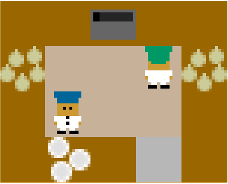
\includegraphics[width=2.8cm]{Figures/overcooked_ai.png} & 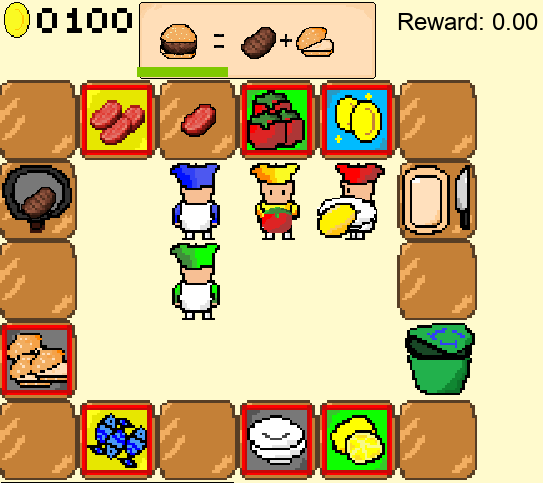
\includegraphics[width=2.8cm]{Figures/complexOvercooked_interface.png} \\[-20pt]
\textbf{4 players} & \ding{55} & \ding{51} \\
\textbf{Dynamic orders} & \ding{55} & \ding{51} \\
\textbf{Synthesis} & \ding{55} & \ding{51} \\
\textbf{LLM control} & \ding{55} & \ding{51} \\
\textbf{\# of interactable objects} & \makecell[c]{\\6} & \makecell[c]{\\18} \\
\bottomrule
\end{tabularx}
\end{table}


In this paper, we introduce \textit{ComplexOvercooked}, a MARL environment that highly replicates the mechanics of the real Overcooked game. Using this environment, dynamic task objectives such as order types, quantities, and durations can be easily configured. Compared to the popular \textit{Overcooked-AI}, \textit{ComplexOvercooked} features more complex game logic (e.g., diverse order synthesis paths), a wider variety of interactive objects, and supports cooperative training for up to four agents (Table \ref{tab:overcooked_comparison}). To demonstrate the potential of this environment in human-agent collaboration tasks, we have integrated control interfaces for both humans and LLMs, enabling easy data collection and the use of LLMs to enhance agent capabilities. We benchmarked the environment using classical MARL algorithms, demonstrating that the environment offers expandable capability boundaries for MARL algorithms. Our contributions can be summarized as follows:
\begin{enumerate}
\item We propose a novel dynamic-objective MARL environment, \textit{ComplexOvercooked}, which faithfully replicates the configurations of the Overcooked game. It is user-friendly, highly configurable, and designed to push the boundaries of cooperative agent capabilities.
\item We integrate multiple control interfaces in \textit{ComplexOvercooked}, including keyboard, model-free RL agent, and model-based LLM controls. This enables seamless collection of human player data, facilitating research on human-agent collaboration algorithms and cooperative LLM algorithms.
\item We benchmark the performance of classical MARL algorithms in various custom layouts of \textit{ComplexOvercooked}. Our experiments demonstrate the potential for enhancing MARL algorithm performance in this environment, highlighting its value as a benchmark for future research.
\end{enumerate}

% Training collaborative agents is a highly popular direction in the field of artificial intelligence. A capable collaborative agent can enhance collaborative performance, influence human behavior \cite{hong2023learning}, and achieve alignment with human values \cite{yuan2022situ} when working alongside humans to accomplish complex tasks. Currently, the training of collaborative agents based on deep reinforcement learning (DRL) primarily relies on the following environments: \textit{Overcooked} \cite{carroll2019utility}, Hanabi \cite{bard2020hanabi}, Multi-Agent Particle Environment (MPE) \cite{lowe2017multi}, Google Research Football (GRF) \cite{kurach2020google} and Starcraft Multi-Agent Challenge(SMAC) \cite{vinyals2017starcraft,samvelyan2019starcraft}. 

% Previous studies are based on the original \textit{Overcooked} game, and these works mainly include the following aspects: zero-short coordination (ZSC) \cite{yu2023learning,zhao2023maximum,strouse2021collaborating,li2023cooperative}, human-AI collaboration \cite{carroll2019utility,strouse2021collaborating,hong2023learning}, robustness analysis of collaborative agents\cite{knott2021evaluating}, and the application of large language models (LLM) in Collaboration \cite{wen2022multi,zhang2023proagent,guan2023efficient,zhu2023madiff}. Although these studies propose algorithms that perform well in original \textit{Overcooked}, they make the improvement margin small\cite{yu2023learning}, which is disadvantageous for the development of collaborative agents.

% The original \textit{Overcooked} environment limits the training of collaborative agents for the following main reasons: Firstly, the game logic is simplified compared to the real \textit{Overcooked} game. \textit{Overcooked} is actually a multiplayer, multitask cooperative game, with up to four players. In it, agents may need to finish multiple orders simultaneously, and multiple agents must have a sense of division of labor and task allocation when completing tasks. These capabilities are not sufficiently reflected in the original \textit{Overcooked} environment. In many \textit{Overcooked} game layouts, one player can do the work of two, and the presence of a companion can actually interfere with an individual agent's actions and path planning. Furthermore, the tasks in \textit{Overcooked} are relatively simple. For example, to make onion soup, one just needs to put three onions in a pot, cook, and serve it to serving area. This results in a rather monotonous workflow of cooperation between agents, where typically one agent places raw onions in the pot while another delivers the soup with a plate. More diverse workflow of cooperation would better test the coordination and collaboration between agents and are beneficial for training agents with superior cooperative abilities.

% 我们提出一个新颖的多人协同的,多任务的overcook\_pygame环境,这个环境更接近真实的overcook游戏。如下图1中所示,智能体需要在规定时间内完成多个特定任务,每道菜的合成路径在上方的任务栏中显示,例如:完成一个番茄牛肉汉堡的过程可能是:将番茄切好,将牛肉放在平底锅中煮熟,在用汉堡和切好的番茄以及煮熟的牛肉合成最终的番茄牛肉汉堡。此外,本环境引入了垃圾回收机制,因为可能有些菜可能未再规定时间内完成,可将其倒入垃圾桶,从而不占桌面空间。总的来说,和之前被广泛使用的合作环境相比,overcook_pygame带来了以下挑战:首先,overcook_pygame是多任务的,同一时间有多个任务需要完成,这有利于研究智能体的信度分配和行为偏好,其次是任务流程复杂多样,完成特定任务的方式可能有多种。overcook_pygame具有高度的可塑性 scalability,玩家可以轻易的修改地图元素,智能体数量和任务类别,任务时间等。此外,我们还提供了大模型的接口便于AI-AI或者人与AI的通讯以实现更好的合作效能。

% We propose a novel multiplayer, multitasking \textit{Overcooked pygame} environment that closely resembles the real \textit{Overcooked} game. As shown in Figure \ref{fig:intro}, agents must complete multiple specific tasks within a limit time. The synthesis steps for each order is displayed in the task menu above. For example, the process of making a \textit{ACtoamtocookedbeefhamburger} might involve chopping tomatoes, cooking beef in a frying pan, and then combining the burger with chopped tomatoes and cooked beef to make the final \textit{ACtoamtocookedbeefhamburger}. Additionally, our environment introduces a garbage recycling mechanism, as some dishes may not be completed within the allotted time and can be dumped into the trash, thereby not occupying table space. Overall, compared to other cooperative environments, \textit{Overcooked pygame} presents the following challenges: Firstly, \textit{Overcooked pygame} is multi-tasking, with multiple tasks to be completed simultaneously, which facilitates research on agent's trust allocation and behavior preferences. Secondly, the task flows are complex and diverse, with multiple possible ways to complete specific tasks. \textit{Overcooked pygame} possesses a high degree of scalability and provides interfaces for large language models (LLM) to facilitate AI-AI or human-AI communication for an improved collaborative performance.

